
\subsection{The plaquette at weak coupling: second moments without the
logarithm, Wilson loops, and the Villain torus}\label{rDtwo:sec}

Throughout this subsection $G=\SU(2)$ unless said otherwise, $\Lambda=
\Lambda_L$ is the torus, $E$ and $P$ are its $4L^4$ links and $6L^4$
plaquettes, $dU$ is normalised Haar measure, and for a plaquette $p$
\[
s_p=1-\tfrac12\Tr U_p\in[0,2],\qquad h_p=2-\Tr U_p=2s_p .
\]
The Wilson weight of Sec.~\ref{ssec:averaged} is $\varphi(U)=e^{-2\beta
(2-\Tr U)}=e^{-bs_p}$ with $b=4\beta$, the conventional coupling $\beta_W$ of the
introduction. For couplings $c=(c_p)_{p\in P}$, $c_p\ge0$, put
$Z(c)=\int_{G^E}\prod_pe^{-c_ps_p}\,dU$ and $Z_L(b)=Z(c)$ when all $c_p=b$,
so that $\mu$ has density $e^{-bS}/Z_L(b)$ with $S=\sum_ps_p$. For $a>0$ let
\[
I(a)=\int_Ge^{-a(1-\frac12\Tr U)}\,dU=\frac2\pi\int_0^\pi e^{-a(1-\cos t)}
\sin^2t\,dt
\]
be the single-plaquette integral (Weyl's formula, $\Tr U=2\cos t$). All
results of this subsection are statements about finite tori; none of them
asserts $\mathrm{BP}(n,\varpi)$ for the Wilson measure, which is a
statement about every real $f\in\mathcal A$ (Definition~\ref{def:avgcube}),
and none bears on condition (D), on $(\mathrm U)$ of
Definition~\ref{rD:U} or on a mass gap.

\subsubsection{Two-sided bounds on the free energy with the same leading
coefficient}

\begin{lemma}[the single-plaquette integral]\label{rDtwo:I}
For every $a>0$,
$\sqrt{2/\pi}\,a^{-3/2}(1-\frac3{4a})\le I(a)\le\sqrt{2/\pi}\,a^{-3/2}$.
\end{lemma}

\begin{proof}
With $u=1-\cos t$, $\sin^2t\,dt=\sqrt{u(2-u)}\,du$ and $I(a)=\frac2\pi
\int_0^2e^{-au}\sqrt{u(2-u)}\,du$. Since $\sqrt{2-u}\le\sqrt2$ and
$\int_0^\infty e^{-au}\sqrt u\,du=\frac{\sqrt\pi}2a^{-3/2}$, the upper bound
follows. Since $\sqrt{2-u}\ge\sqrt2(1-u/2)$ on $[0,2]$ and $e^{-au}\sqrt u
(1-u/2)\le0$ on $[2,\infty)$,
\[
\begin{split}
I(a)&\ge\frac{2\sqrt2}\pi\int_0^\infty e^{-au}\sqrt u\Bigl(1-\frac u2\Bigr)du\\
&=\frac{2\sqrt2}\pi\Bigl(\frac{\sqrt\pi}2a^{-3/2}-\frac{3\sqrt\pi}8a^{-5/2}
\Bigr).\qedhere
\end{split}
\]
\end{proof}

\begin{lemma}[gauge fixing on the torus]\label{rDtwo:gauge}
Let $G$ be a compact group, $T\subset E$ a maximal tree of $\Lambda_L$
($\lvert T\rvert=L^4-1$) and $f$ an integrable gauge-invariant function on
$G^E$. Then $\int_{G^E}f\,dU=\int_{G^{E\setminus T}}f(V,1_T)\,dV$, where
$(V,1_T)$ equals $V$ on $E\setminus T$ and the identity on $T$.
\end{lemma}

\begin{proof}
As in Lemma~\ref{lem:gaugefix}, with the tree in place of the forest: fix a
root $x_0$; the map $(g,V)\mapsto g\cdot(V,1_T)$ from $\{g\in G^\Lambda:
g_{x_0}=1\}\times G^{E\setminus T}$ to $G^E$, $(g\cdot U)_{(x,\mu)}=g_xU_{(x,
\mu)}g_{x+e_\mu}^{-1}$, is a bijection, since the conditions $(g^{-1}\cdot
U)_e=1$, $e\in T$, determine $g$ uniquely along the tree from the root and
then $V=(g^{-1}\cdot U)\vert_{E\setminus T}$. Ordering the links of $T$ from
the root, each $U_e$ is a left and right translate of one new variable
($g_x$ for $e\in T$, $V_e$ for $e\notin T$) by previously determined ones,
so the map preserves Haar measure; the numbers of factors agree, $(L^4-1)+
(3L^4+1)=4L^4$. Gauge invariance gives $f(g\cdot(V,1_T))=f(V,1_T)$, and
integrating out $g$ gives the claim.
\end{proof}

We use the maximal tree $T$ of the links $(y,0)$ with $y_1=y_2=y_3=0$,
$y_0\le L-2$; $(y,1)$ with $y_2=y_3=0$, $y_1\le L-2$; $(y,2)$ with $y_3=0$,
$y_2\le L-2$; and $(y,3)$ with $y_3\le L-2$ (coordinates in $\{0,\dots,
L-1\}$), and the four closing links $u_\mu=((L-1)e_\mu,\mu)$. Put $F=T\cup
\{u_0,\dots,u_3\}$, $\lvert F\rvert=L^4+3$.

\begin{lemma}[the lower bound]\label{rDtwo:jensen}
Let $b>0$ and $c_p\in[0,b]$ for all $p$. Then $Z(c)\ge I(6b)^{3L^4+1}$.
\end{lemma}

\begin{proof}
By Lemma~\ref{rDtwo:gauge}, $Z(c)=\int_{G^N}\prod_pe^{-c_ps_p(V,1_T)}\,dV$,
$N=3L^4+1$. Let $\nu_a$ have density $\rho_a(W)=e^{-a(1-\frac12\Tr W)}/I(a)$,
a class function, and write $dV=\prod_e\rho_a(V_e)^{-1}d\nu_a(V_e)$. By
Jensen's inequality for the concave logarithm,
\[
\log Z(c)\ge\E_{\nu_a^{\otimes N}}\Bigl[-\sum_pc_ps_p-\sum_{e\notin T}\log
\rho_a(V_e)\Bigr].
\]
Put $g(a)=\E_{\nu_a}(1-\frac12\Tr W)$, so $-\E\log\rho_a(V_e)=ag(a)+\log
I(a)$. Let $k_p\le4$ be the number of links of $p$ outside $T$; in $(V,1_T)$
the holonomy $U_p$ is a product of $k_p$ independent factors $V_e^{\pm1}$
with conjugation-invariant laws, so by Schur's lemma each factor has matrix
expectation $(1-g(a))\mathbf 1$ (also for $V_e^{-1}$, as $\Tr V^{-1}=\Tr V$ on
$\SU(2)$), hence $\E s_p=1-(1-g(a))^{k_p}\le k_pg(a)$ (Bernoulli if $g\le1$,
trivially if $g>1$). Every link lies in six plaquettes, so $\sum_pk_p=6N$,
and with $c_p\le b$,
\[
\log Z(c)\ge N\log I(a)+Ng(a)(a-6b).
\]
Take $a=6b$.
\end{proof}

\begin{lemma}[shelling]\label{rDtwo:shell}
Let $(e_1,p_1),\dots,(e_M,p_M)$ be link--plaquette pairs with $e_j\in p_j$
and $e_k\notin p_j$ whenever $k>j$. Then $Z(c)\le\prod_{j=1}^MI(c_{p_j})$
for all couplings $c_p\ge0$, and necessarily $M\le3L^4-3$.
\end{lemma}

\begin{proof}
Integrate $U_{e_M}$ first. Among $p_1,\dots,p_M$ only $p_M$ contains $e_M$;
drop the weights $e^{-c_ps_p}\le1$ of the other plaquettes through $e_M$. By
cyclicity $s_{p_M}=1-\frac12\Tr(U_{e_M}^{\pm1}W)$ with $W$ the product of the
other three links of $p_M$, and $\int_Ge^{-c(1-\frac12\Tr(U^{\pm1}W))}dU=I(c)$
by the invariance of Haar measure under inversion and translation. The
remaining integrand involves $p_1,\dots,p_{M-1}$ and plaquettes not
containing $e_M$; repeat with $e_{M-1}$, and so on; after $M$ steps all
remaining weights are at most $1$. For the bound on $M$: the $1$-chains
$\partial p_1,\dots,\partial p_M$ are linearly independent, since in a
vanishing combination the largest index $j$ with nonzero coefficient has
$e_j\in p_j$ and $e_j\notin p_i$ for $i<j$, so the coefficient of $e_j$ is
$\pm$ that of $\partial p_j$. Hence $M\le\operatorname{rank}\partial_2=\dim
\ker\partial_1-\dim H_1(\Lambda_L;\R)=(4L^4-(L^4-1))-4=3L^4-3$, as
$\operatorname{rank}\partial_1=L^4-1$.
\end{proof}

\begin{lemma}[an explicit shelling]\label{rDtwo:shellexplicit}
For every $L\ge2$ there is a sequence as in Lemma~\ref{rDtwo:shell} with
$M=3L^4-3$, whose links are exactly those of $E\setminus F$, and whose
plaquettes in the plane $\{1,2\}$ are the $L^3-L$ plaquettes $(y,12)$ with
$y_3=0$ and $(y_1,y_2)\ne(0,L-1)$. When $L$ is even, exactly
$m_O=\frac L2(L^2-1)<L^3/2$ of them have $y_0$ and $y_3$ even.
\end{lemma}

\begin{proof}
Read the condition in the order $j=1,2,\dots$: $p_j$ contains $e_j$ and
otherwise only links of $F\cup\{e_1,\dots,e_{j-1}\}$; so the sequence is
built by adding links, each new link completing a plaquette whose other
three links are present, starting from $F$. Write $(y,\mu\nu)$ for
plaquettes and $(y,\mu)$ for links.

\emph{Stage 1, the $2$-torus $\{(x_0,x_1,\ast,\ast)\}$, given that it
contains $(y,2)$ with $y_3=0$ (all $y_2$), $(y,3)$ with $y_3\le L-2$ (all
$y_2$), and $(x_0,x_1,0,L-1,3)$.} For $x_3=0,\dots,L-2$ and all $x_2$ the
plaquette $(y,23)$, $y=(x_0,x_1,x_2,x_3)$, has $(y,2)$ (by induction on
$x_3$), $(y+e_2,3)$, $(y,3)$ present and adds $(y+e_3,2)$. Then for $x_2=0,
\dots,L-2$ the plaquette $(y,23)$ with $y=(x_0,x_1,x_2,L-1)$ has $(y,2)$,
$(y,3)$ (by induction on $x_2$ from the closing link) and $(y+e_3,2)=(x_0,x_1,
x_2,0,2)$ present and adds $(y+e_2,3)$. This adds $L^2-1$ links, all links
of the $2$-torus, with $L^2-1$ distinct plaquettes of the plane $\{2,3\}$.

\emph{Stage 2, the $3$-torus $\{(x_0,\ast,\ast,\ast)\}$, given that it
contains $(y,1)$ with $y_2=y_3=0$ (all $y_1$), $(y,2)$ with $y_3=0$, $y_2\le
L-2$, $(y,3)$ with $y_3\le L-2$, and $(x_0,0,0,L-1,3)$, $(x_0,0,L-1,0,2)$.}
Run Stage 1 in the slice $x_1=0$. For all $x_1$ and $x_2\le L-2$ the
plaquette $(y,12)$, $y=(x_0,x_1,x_2,0)$, adds $(y+e_2,1)$; for $x_3\le L-2$
and all $x_1,x_2$ the plaquette $(y,13)$ adds $(y+e_3,1)$; so all $(y,1)$
are present. For $x_1=L-1,L-2,\dots,1$ in this order, $(y,12)$ with $y=(x_0,
x_1,L-1,0)$ adds $(y,2)$ and $(y,13)$ with $y=(x_0,x_1,0,L-1)$ adds $(y,3)$,
using the slice $x_1+1$ (the slice $0$ for $x_1=L-1$). Each slice $x_1\ne0$
now satisfies the hypothesis of Stage 1, which is run in each. Stage 2
adds $(L^2-1)+(L^3-L)+2(L-1)+(L-1)(L^2-1)=2L^3-2$ links, all links of the
$3$-torus, and uses $L(L-1)+(L-1)=L^2-1$ plaquettes of the plane $\{1,2\}$,
all with $y_3=0$ and $(y_1,y_2)\ne(0,L-1)$.

\emph{Stage 3, the torus.} $F$ satisfies the hypothesis of Stage 2 in the
slice $x_0=0$; run Stage 2 there. For $x_1\le L-2$ and all $x_0$ the
plaquette $(y,01)$, $y=(x_0,x_1,0,0)$, adds $(y+e_1,0)$; for $x_2\le L-2$
the plaquette $(y,02)$, $y=(x_0,x_1,x_2,0)$, adds $(y+e_2,0)$; for $x_3\le
L-2$ the plaquette $(y,03)$ adds $(y+e_3,0)$; so all $(y,0)$ are present.
For $x_0=L-1,\dots,1$ the plaquettes $(y,01)$, $(y,02)$, $(y,03)$ with $y=
(x_0,L-1,0,0)$, $(x_0,0,L-1,0)$, $(x_0,0,0,L-1)$ add $(y,1)$, $(y,2)$,
$(y,3)$, using the slice $x_0+1$. Each slice $x_0\ne0$ then satisfies the
hypothesis of Stage 2, which is run in each. In all $(2L^3-2)+(L^4-L)+3(L-1)
+(L-1)(2L^3-2)=3L^4-3$ links are added, the links of $E\setminus F$, and the
plaquettes of the plane $\{1,2\}$ used are $L(L^2-1)=L^3-L$, one in each
slice $x_0$ for each $(y_1,y_2)\ne(0,L-1)$, all with $y_3=0$; for even $L$
those with $y_0$ even number $\frac L2(L^2-1)$. At each step the other three
links of the plaquette were present, which is the condition of
Lemma~\ref{rDtwo:shell}.
\end{proof}

\begin{proposition}[two-sided bounds]\label{rDtwo:freeenergy}
Let $b>1/8$, $c_p\in(0,b]$ for all $p$, and $(e_j,p_j)_{j\le3L^4-3}$ the
sequence of Lemma~\ref{rDtwo:shellexplicit}. Then
\[
\begin{split}
\log Z(c)&\ge(3L^4+1)\Bigl[\tfrac12\log\tfrac2\pi-\tfrac32\log(6b)+\log\Bigl(1-
\frac1{8b}\Bigr)\Bigr],\\
\log Z(c)&\le\sum_{j=1}^{3L^4-3}\Bigl[\tfrac12\log\tfrac2\pi-\tfrac32\log c_{p_j}
\Bigr].
\end{split}
\]
With all $c_p=b$ the two bounds on $\log Z_L(b)$ differ by
\[
2\log\tfrac\pi2+\tfrac92L^4\log6+\tfrac32\log6+6\log b+(3L^4+1)\log\frac{8b}
{8b-1}:
\]
the coefficient of $L^4\log b$ is $-\frac92$ in both, and the residual
$6\log b$ comes from the four links of $F\setminus T$, which no shelling
can use (Lemma~\ref{rDtwo:shell}: $\operatorname{rank}\partial_2=3L^4-3$
because $H_1(\Lambda_L)=\R^4$) and which the lower bound treats as massive.
\end{proposition}

\begin{proof}
Lemmas \ref{rDtwo:jensen}, \ref{rDtwo:shell}, \ref{rDtwo:shellexplicit} and
\ref{rDtwo:I}; in the lower bound $3/(4\cdot6b)=1/(8b)$.
\end{proof}

The upper bound improves~\cite[Lemma~475]{BBLR26}, whose axial gauge uses $3L^3(L-1)$ plaquettes
and the constant $(\pi/2)^{5/2}$, to $3L^4-3$ plaquettes and the constant
$\sqrt{2/\pi}$.

\subsubsection{The first moment of the plaquette without the logarithm}

\begin{theorem}[the plaquette energy]\label{rDtwo:firstmoment}
Let $\beta\ge1$ and $L\ge2$. For every plaquette $p$,
\[
\mu(2-\Tr U_p)\le\frac1\beta\Bigl(1.6+\frac{2\log(4\beta)}{3L^4}\Bigr).
\]
\end{theorem}

\begin{proof}
Put $\Phi(b)=\log Z_L(b)$; then $\Phi'(b)=-\E_bS$, $\Phi''(b)=\Var_b(S)\ge0$,
and convexity gives, for $\theta\in(0,1)$, $\E_bS\le(\Phi(\theta b)-\Phi(b))/
((1-\theta)b)$. By Proposition~\ref{rDtwo:freeenergy} with couplings
$\theta b$ in the upper bound,
\[
\begin{split}
\Phi(\theta b)-\Phi(b)&\le2\log\tfrac\pi2+\tfrac92L^4\log\tfrac6\theta+\tfrac32
(\log6+3\log\theta)\\
&\quad+6\log b+(3L^4+1)\log\frac{8b}{8b-1}.
\end{split}
\]
Take $\theta=1/4$, so that $\frac32(\log6+3\log\theta)+2\log\frac\pi2<0$;
with $\E_bs_p=\E_bS/(6L^4)$ by translation invariance,
\[
\E_bs_p\le\frac1b\Bigl[\log24+\frac23\Bigl(1+\frac1{3L^4}\Bigr)\log\frac{8b}
{8b-1}+\frac{4\log b}{3L^4}\Bigr].
\]
For $b=4\beta\ge4$ and $L\ge2$ the middle term is at most $\frac23\cdot\frac
{49}{48}\log\frac{32}{31}<0.0217$. Since $\mu(2-\Tr U_p)=2\E_bs_p$ and $2/b
=1/(2\beta)$, the bracket is halved: $\frac12\log24<1.5891$ and $\frac12
\cdot0.0217<0.0109$ give the constant $1.6$, and $\frac{2}{b}\cdot\frac
{4\log b}{3L^4}=\frac{2\log(4\beta)}{3L^4\beta}$.
\end{proof}

Theorem~\ref{rDtwo:firstmoment} replaces the bound $(\log\beta+6.11)/\beta$
of Lemma~\ref{lem:bpflat}: the logarithm there came from bounding the free
energy at coupling $\beta/2$ by $\log Z\le0$, while here both free energies
are bounded with the same coefficient of $L^4\log b$, and the only logarithm
left is the global term $6\log b$ divided by the number $6L^4$ of
plaquettes. The weak-coupling value of $\E_bs_p$ is $3/(4b)+O(b^{-2})$, so
the constant $\log24$ is off by a factor of about $4.2$.

\subsubsection{The tail of the plaquette energy and the second moment}

Let $L$ be even. Put $Y=\{y\in\Lambda_L:y_0,y_3\text{ even}\}$, $\lvert Y
\rvert=L^4/4$, and $O=\{(y,12):y\in Y\}$, a set of $L^4/4$ plaquettes. For a
site reflection $\vartheta$ (in a hyperplane $x_\mu=k$, $k\in\Z$) put
$(\vartheta U)_e=U_{\vartheta e}^{\pm1}$, the inverse for the links
perpendicular to the hyperplane, whose orientation is reversed. It maps
plaquettes to plaquettes, and the holonomy of $\vartheta p$ in $\vartheta U$
is a conjugate of $U_p^{\pm1}$.

\begin{lemma}[chessboard estimate]\label{rDtwo:chess}
Let $G$ be a compact group, $\psi\ge0$ a class function on $G$ with
$\psi(U^{-1})=\psi(U)$, and $\mu$ the measure with density proportional to
$\prod_p\psi(U_p)$ on $G^E$. Let $p=(0,12)$ and $\varepsilon\ge0$.
\begin{enumerate}[label=\textup{(\roman*)},leftmargin=*]
\item If $4\mid L$, then $\mu(s_p>\varepsilon)\le\mu\bigl(\bigcap_{q\in O}
\{s_q>\varepsilon\}\bigr)^{4/L^4}$.
\item If $L$ is even, then $\mu(s_p>\varepsilon)\le\mu\bigl(\bigcap_{q\in O}
\{s_q>\varepsilon\}\bigr)^{1/L^4}$.
\end{enumerate}
The same holds for $\{\lvert\theta_p\rvert>\delta\}$ in place of $\{s_p>
\varepsilon\}$ when $G=\U(1)$, $U_p=e^{i\theta_p}$.
\end{lemma}

\begin{proof}
The measure is reflection positive for every reflection in a hyperplane
through sites \cite{OSei78,Sei82}: every plaquette lies in the hyperplane
or on one side of it, the weight factorises as $W_+W_0W_-$ with $W_0\ge0$
a function of the links in the hyperplane and $W_-=\vartheta W_+$ (here
$\psi(U^{-1})=\psi(U)$ and the class property are used), so that for $F$
measurable with respect to the links on the positive side, $\int F\,
\overline{\vartheta F}\prod_p\psi(U_p)\,dU=\int W_0\bigl\lvert\int FW_+\bigr
\rvert^2\ge0$, as $\vartheta$ preserves Haar measure. (i) Tile the torus by
the $L^4/4$ blocks $y+[-1,1]\times[0,1]\times[0,1]\times[-1,1]$, $y\in Y$;
the separating hyperplanes $x_0\in2\Z+1$, $x_3\in2\Z+1$, $x_1\in\Z$, $x_2\in
\Z$ pass through sites, and the number of blocks in each direction, $L/2$
or $L$, is even. The chessboard estimate \cite[Sect.~2]{FILS78},
\cite[Sect.~5.3]{Bis09} then gives $\mu(f)\le\mu(\prod_{y\in Y}f^{(y)})^{4/
L^4}$ for every bounded $f\ge0$ of the links with both endpoints in the
block of $0$, where $f^{(y)}$ is the image of $f$ under the element of the
group generated by the reflections that carries the block of $0$ to that
of $y$ (for an even number of blocks in each direction this element is
unique on blocks: a translation by $y_\mu$ when $y_\mu\equiv0\bmod4$ in the
directions $0,3$, resp.\ $y_\mu$ even in the directions $1,2$, otherwise the
reflection in $x_\mu=y_\mu/2$, resp.\ $x_\mu=(y_\mu+1)/2$). For $f=1_{\{s_p>
\varepsilon\}}$ this element carries the plaquette $(0,12)$ to $(y,12)$, up
to orientation, so $f^{(y)}=1_{\{s_{(y,12)}>\varepsilon\}}$ by the invariance
of the trace under conjugation and inversion. (ii) Use the unit blocks $y+
[0,1]^4$, $y\in\Lambda_L$, $L$ even; the chessboard estimate gives $\mu(f)
\le\mu(\prod_{y\in\Lambda_L}f^{(y)})^{1/L^4}$, and the element carrying the
block of $0$ to that of $y$ carries $(0,12)$ to $(y',12)$ with $y'_\mu=y_\mu$
for $y_\mu$ even and $y'_\mu=y_\mu+1$ for $y_\mu$ odd in the directions
$0,3$, and to $(y,12)$ up to orientation in the directions $1,2$; so each
indicator $1_{\{s_q>\varepsilon\}}$, $q\in O$, appears four times in the
product, which is therefore $1_{\bigcap_{q\in O}\{s_q>\varepsilon\}}$.
\end{proof}

The $2\times1\times1\times2$ blocks of (i) are needed because a block of
side $2$ in the directions $0,3$ keeps the orbit of $(0,12)$ at one
plaquette in four; for $L\equiv2\bmod4$ the number $L/2$ of such blocks is
odd and the chessboard estimate does not apply to them (the reflection in
$x_0=L/2$ maps a block onto itself), so (ii) is used instead.

\begin{theorem}[the tail of the plaquette energy]\label{rDtwo:tail}
Let $\beta\ge1$, $L\ge8$ even, $b=4\beta$, $p$ a plaquette, $\varepsilon\ge
0$ and $\lambda\in(0,1)$. Put
\[
\begin{split}
A_\lambda&=18\log6+12\log\frac{8b}{8b-1}+\frac3L\log\frac1{1-\lambda}\\
&\quad+\frac1{L^4}\Bigl[24\log b+6\log6+8\log\frac\pi2+4\log\frac{8b}{8b-1}
\Bigr],
\end{split}
\]
and $\kappa_L=1$ if $4\mid L$, $\kappa_L=4$ if $L\equiv2\bmod4$. Then
\[
\mu(s_p>\varepsilon)\le\exp\bigl((-\lambda b\varepsilon+A_\lambda)/\kappa_L
\bigr),
\]
and $A_{9/10}\le33.5+24L^{-4}\log(4\beta)$.
\end{theorem}

\begin{proof}
By symmetry $p=(0,12)$. On $\{s_q>\varepsilon\}$, $1\le e^{\lambda b(s_q-
\varepsilon)}$, so by Lemma~\ref{rDtwo:chess}
\[
\mu(s_p>\varepsilon)^{\kappa_LL^4/4}\le e^{-\lambda b\varepsilon\lvert O\rvert}
\,\frac{Z(c)}{Z_L(b)},
\]
where $c_q=(1-\lambda)b$ for $q\in O$ and $c_q=b$ for $q\notin O$.
In the shelling of Lemma~\ref{rDtwo:shellexplicit}, $m_O=\frac L2(L^2-1)$
plaquettes lie in $O$ and the other $3L^4-3-m_O$ have coupling $b$; with the
lower bound of Lemma~\ref{rDtwo:jensen} for $Z_L(b)$,
Proposition~\ref{rDtwo:freeenergy} gives
\[
\begin{split}
\log\frac{Z(c)}{Z_L(b)}&\le2\log\tfrac\pi2+\tfrac92L^4\log6+\tfrac32\log6+6
\log b\\
&\quad+\tfrac32m_O\log\frac1{1-\lambda}+(3L^4+1)\log\frac{8b}{8b-1}.
\end{split}
\]
Multiplying by $4/(\kappa_LL^4)$ and using $\lvert O\rvert=L^4/4$ and
$6m_O/L^4<3/L$ gives the bound. For $\lambda=9/10$, $b\ge4$ and $L\ge8$:
$18\log6<32.2517$, $12\log\frac{32}{31}<0.3810$, $\frac38\log10<0.8635$ and
$8^{-4}(6\log6+8\log\frac\pi2+4\log\frac{32}{31})<0.0036$, in all less than
$33.5$.
\end{proof}

\begin{theorem}[the second moment of the plaquette]\label{rDtwo:secondmoment}
Let $\beta\ge1$ and $L\ge8$ even, $\ell=L^{-4}\log(4\beta)$, and $C_L=368$
if $4\mid L$, $C_L=439$ if $L\equiv2\bmod4$. For every plaquette $p$,
\[
\Var_\mu(\Tr U_p)\le\mu\bigl((2-\Tr U_p)^2\bigr)\le\frac{C_L\,(1+\ell)^2}
{\beta^2}.
\]
\end{theorem}

\begin{proof}
Put $\lambda=9/10$, $A=33.5+24\ell$, $\kappa=\kappa_L$, so that $\mu(s_p>
\varepsilon)\le\min(1,e^{(A-\lambda b\varepsilon)/\kappa})$. With $\varepsilon
_0=A/(\lambda b)$,
\[
\begin{split}
\mu(s_p^2)&=\int_0^22\varepsilon\,\mu(s_p>\varepsilon)\,d\varepsilon\\
&\le\varepsilon_0^2+\int_{\varepsilon_0}^\infty2\varepsilon
e^{-\lambda b(\varepsilon-\varepsilon_0)/\kappa}d\varepsilon\\
&=\frac{A^2+2\kappa A+2\kappa^2}{\lambda^2b^2}.
\end{split}
\]
For $x\ge0$, $(A_1+x)^2+2\kappa(A_1+x)+2\kappa^2\le(A_1^2+2\kappa A_1+2
\kappa^2)(1+x/A_1)^2$ (expand both sides), and $24\ell/33.5\le\ell$; so with
$A_1=33.5$, $A^2+2\kappa A+2\kappa^2\le(A_1^2+2\kappa A_1+2\kappa^2)(1+\ell)
^2$. Finally $\mu((2-\Tr U_p)^2)=4\mu(s_p^2)$, $b=4\beta$, and $(A_1^2+2A_1+
2)/(4\lambda^2)<367.7$, $(A_1^2+8A_1+32)/(4\lambda^2)<439$.
\end{proof}

\begin{remark}[the residual $\ell$]\label{rDtwo:zeromodes}
The factor $(1+\ell)^2$, $\ell=L^{-4}\log(4\beta)$, is the only trace of
$\beta$ beyond $\beta^{-2}$. It comes from the term $6\log b$ of
Proposition~\ref{rDtwo:freeenergy}, the mismatch between the $3L^4-3$
plaquettes a shelling can use and the $3L^4+1$ links the lower bound treats
as massive, that is from $H_1(\Lambda_L)=\R^4$: the flat connections of the
torus (commuting holonomies around the four cycles) are zero modes of the
action, and neither bound integrates over them. The chessboard estimate
raises the ratio of partition functions to the power $4/L^4$, so this
global term enters the tail as $b^{24/L^4}$. For $\log(4\beta)\le L^4$ the
bound reads $\mu((2-\Tr U_p)^2)\le4C_L/\beta^2$, and as $L\to\infty$ at
fixed $\beta$ it tends to $C_L/\beta^2$. Removing $\ell$ would require a
lower bound on $Z_L(b)$ with the exact power of $b$, which is not
determined here.
\end{remark}

\begin{corollary}[a $\beta$-independent constant for the plaquette traces]
\label{rDtwo:bpplaquette}
Let $\beta\ge11$, $n\ge2$, $L\ge2n+4$ even, $\ell=L^{-4}\log(4\beta)$, $C_L$
as in Theorem~\ref{rDtwo:secondmoment}. For every plaquette $p$ and every
link $e\in p$,
\begin{enumerate}[label=\textup{(\roman*)},leftmargin=*]
\item $\mu(\Var_\mu(\Tr U_p\mid\mathcal F_e))\ge1/(1200\beta^2)$;
\item $\mathcal E_n(\Tr U_p)\ge\mu(\Var_\mu(\Tr U_p\mid\mathcal F_e))$, hence
\[
\mathcal E_n(\Tr U_p)\ge\frac1{1200\beta^2}\ge
\frac{\Var_\mu(\Tr U_p)}{1200\,C_L\,(1+\ell)^2}.
\]
\end{enumerate}
In particular the inequality of $\mathrm{BP}(n,\varpi)$ holds for the
functions $\Tr U_p$ with $\varpi=1/(1200C_L(1+\ell)^2)$, and with $\varpi=
1/(1.77\cdot10^6)$ for $4\mid L$, $\varpi=1/(2.11\cdot10^6)$ for $L\equiv2
\bmod4$, whenever $\log(4\beta)\le L^4$, uniformly in $\beta$, $L$, $n$ and
$p$. This is a statement about these functions only: by
Theorem~\ref{thm:bpfixed}(ii), $\mathrm{BP}(n,\varpi)$ itself fails on
$\Lambda_{2n+4}$ unless $\varpi\le38400n^4(\log\beta+6.11)/\beta$, so no
$\beta$-independent constant holds for all of $\mathcal A$ at fixed $n$.
\end{corollary}

\begin{proof}
(i) The proof of Proposition~\ref{rD:plaquette}(i) gives $\Var_\mu(\Tr U_p
\mid\mathcal F_e)\ge1/(600\beta^2)$ on $\{a\ge6\}$, $a=4\beta\lvert w\rvert$,
and on $\{a<6\}$ it gives $\sum_{p'\ni e}s_{p'}=\frac12\sum_{p'\ni e}(2-\Tr
U_{p'})>6-\frac3{2\beta}$, so that $s_{p'}>1-\frac1{4\beta}$ for one of the
six plaquettes $p'\ni e$ (this step did not use $\beta\ge100$). By Markov's
inequality, Theorem~\ref{rDtwo:firstmoment} and the equivalence of all
plaquettes,
\[
\mu(a<6)\le\frac{6\,\mu(s_p)}{1-1/(4\beta)}\le\frac{6\bigl(0.8+\frac{\log(4
\beta)}{3L^4}\bigr)}{\beta-\frac14}\le\frac12
\]
for $\beta\ge11$ and $L\ge8$: the middle expression is $0.447$ at $\beta=11$,
$L=8$, decreases in $L$, and decreases in $\beta$ since its logarithmic
derivative is negative. Hence $\mu(\Var_\mu(\Tr U_p\mid\mathcal F_e))\ge\frac
12\cdot\frac1{600\beta^2}$.

(ii) In Sec.~\ref{ssec:averaged}, $V_x$ is the set of links with base point
in $x+[0,n)^4$, so a link $e=(y,\mu)$ lies in $V_x$ for exactly the $n^4$
values $x\in y-[0,n)^4$, distinct residues as $L\ge n+2$. For each of them
$\mathcal F_{V_x}\subset\mathcal F_e$, hence $\mu((f-\mathcal P_xf)^2)\ge\mu(
\Var_\mu(f\mid\mathcal F_e))$ for every $f$, as in the proof of
Proposition~\ref{rD:local}; dropping the other $x$ gives $\mathcal E_n(f)\ge
n^{-4}\cdot n^4\,\mu(\Var_\mu(f\mid\mathcal F_e))$. Combine with (i) and
Theorem~\ref{rDtwo:secondmoment}; $1200\cdot4\cdot368<1.77\cdot10^6$ and
$1200\cdot4\cdot439<2.11\cdot10^6$.
\end{proof}

This is the bound asked for in Remark~\ref{rD:plaqloss}, with $C=C_L(1+\ell
)^2$. The argument of (ii) is general: $\mathcal E_n(f)\ge\max_e\mu(\Var_\mu(f
\mid\mathcal F_e))$ for every $f\in L^2(\mu)$, which removes the factor
$((n-1)/n)^2$ of Proposition~\ref{rD:plaquette}(iii) (that factor counted the
cubes containing all four links of $p$); the threshold $\beta\ge100$ there
becomes $\beta\ge11$. Proposition~\ref{rD:plaquette}(ii), (iii) are
superseded for $\beta\ge11$ and even $L\ge8$.

\subsubsection{Wilson loops of fixed size}

For a closed lattice path $\gamma=(x_0,x_1,\dots,x_m=x_0)$ let $W_\gamma=
U_{(x_0,x_1)}\cdots U_{(x_{m-1},x_m)}$, with $U_{(x,x+e_\mu)}=U_{(x,\mu)}$
and $U_{(x+e_\mu,x)}=U_{(x,\mu)}^{-1}$; $W$ is multiplicative under
concatenation, $W_{\gamma^{-1}}=W_\gamma^{-1}$, and is unchanged by inserting
or removing a backtracking $(x,y,x)$. Let $\theta(U)=\arccos(\frac12\Tr U)
\in[0,\pi]$, the geodesic distance from $\mathbf 1$ in the bi-invariant
metric of $S^3$, so that $\theta(gUg^{-1})=\theta(U)=\theta(U^{-1})$ and
$\theta(UV)\le\theta(U)+\theta(V)$.

\begin{lemma}[lassos]\label{rDtwo:lasso}
Let $1\le r\le L-1$, $\{\mu,\nu\}$ a plane, $R$ the set of the $r^2$
plaquettes $(y+ie_\mu+je_\nu,\mu\nu)$, $0\le i,j<r$, and $\gamma$ the
boundary loop of their union, based at $y$. Then $W_\gamma=\prod_{p\in R}
g_pU_p^{\pm1}g_p^{-1}$ in a suitable order, with $g_p$ the holonomy of a
path from $y$ to a corner of $p$; consequently $\theta(W_\gamma)\le\sum_{p
\in R}\theta(U_p)$.
\end{lemma}

\begin{proof}
Add the plaquettes row by row ($j$ outer, $i$ inner). After each step the
union $R_k$ is a staircase region (full rows below a partial row) with
boundary a simple closed curve $\gamma_k$ through $y$; the next plaquette
$p$ meets $R_k$ along one or two consecutive edges, forming a path $\sigma
\subset\gamma_k$, and $\gamma_{k+1}$ replaces $\sigma$ by the complementary
path $\tau$ of $\partial p$. Writing $\gamma_k=\alpha\sigma\alpha'$ from $y$,
$\gamma_{k+1}=\alpha\tau\alpha'\sim(\alpha\tau\sigma^{-1}\alpha^{-1})(\alpha
\sigma\alpha')$ after inserting the backtrack $\alpha^{-1}\alpha$, so
$W_{\gamma_{k+1}}=gU_p^{\pm1}g^{-1}W_{\gamma_k}$ with $g=W_\alpha$ times the
holonomy along $\partial p$ from the start of $\sigma$ to the corner of $p$.
Induction gives the product formula; the triangle inequality and the
invariance of $\theta$ give the angle bound. For $r\le L-1$ the $r^2$
plaquettes are distinct and the region embeds in the torus.
\end{proof}

\begin{theorem}[Wilson loops of size $r$]\label{rDtwo:loops}
Let $\beta\ge11$, $n\ge2$, $L\ge2n+4$ even, $\ell$, $C_L$ as above, $\gamma$
the boundary of an $r\times r$ square of plaquettes, $1\le r\le L-1$, $e$ a
link of $\gamma$, $W=W_\gamma$.
\begin{enumerate}[label=\textup{(\roman*)},leftmargin=*]
\item $\mu(\Var_\mu(\Tr W\mid\mathcal F_e))\ge1/(1200\beta^2)$; this holds
for every closed path through $e$ exactly once, of any shape.
\item $\Var_\mu(\Tr W)\le\mu\bigl((2-\Tr W)^2\bigr)\le\frac{\pi^4}{16}\,
r^8\,C_L(1+\ell)^2/\beta^2$, which is at most $2241\,r^8(1+\ell)^2/\beta^2$
for $4\mid L$ and $2673\,r^8(1+\ell)^2/\beta^2$ for $L\equiv2\bmod4$.
\item $\mathcal E_n(\Tr W)\ge\mu(\Var_\mu(\Tr W\mid\mathcal F_e))$, hence
\[
\mathcal E_n(\Tr W)\ge\frac1{1200\beta^2}\ge
\frac{\Var_\mu(\Tr W)}{1200\cdot\frac{\pi^4}{16}C_L\,r^8(1+\ell)^2};
\]
the denominator is at most $2.69\cdot10^6\,r^8(1+\ell)^2$ for $4\mid L$ and
$3.21\cdot10^6\,r^8(1+\ell)^2$ for $L\equiv2\bmod4$.
\end{enumerate}
\end{theorem}

\begin{figure}[t]
\centering
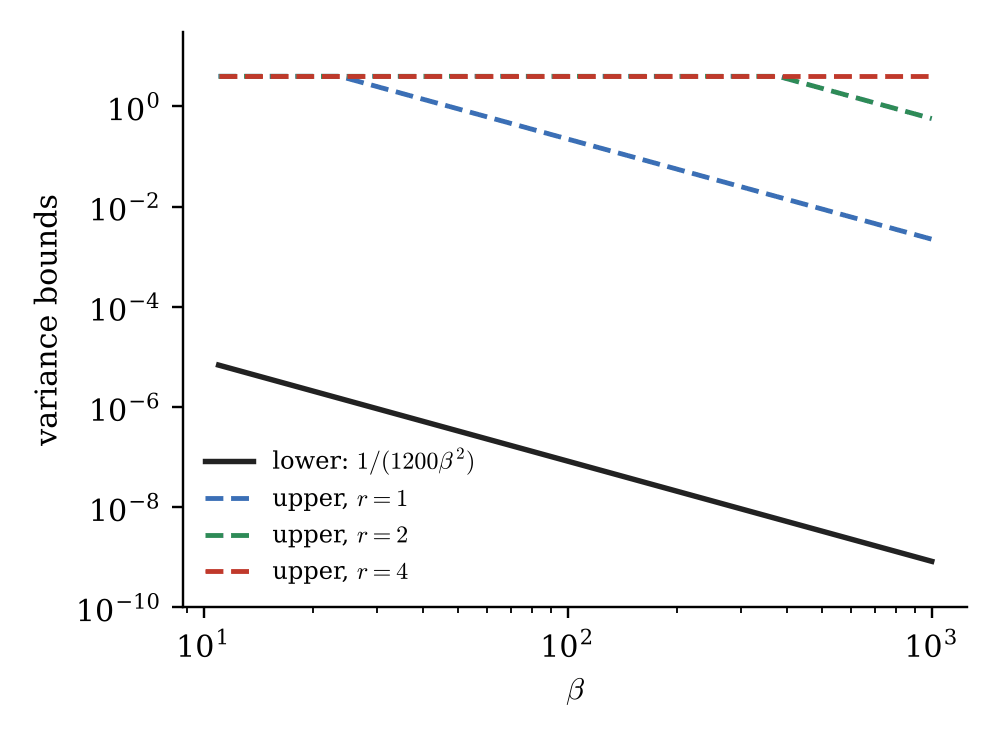
\includegraphics[width=\columnwidth]{figures/fig_wilson.png}
\caption{The two bounds of Theorem~\ref{rDtwo:loops} for $4\mid L$ and
$\ell\to0$: the lower bound $1/(1200\beta^2)$ on the averaged conditional
variance of $\Tr W$ at one link of the loop, and the upper bound
$\min(4,2241\,r^8/\beta^2)$ on the variance of $\Tr W$ for loops of side
$r=1,2,4$. Both scale as $\beta^{-2}$, so their ratio does not depend on
$\beta$.}
\label{fig:wilson}
\end{figure}

\begin{proof}
(i) As in the proof of Proposition~\ref{rD:plaquette}(i), the conditional
law of $U_e$ given $\mathcal F_e$ is $\nu_{a,\hat w}$ with $a=4\beta\lvert w
\rvert$, and since $e$ occurs once in $\gamma$, $\Tr W=\Tr(U_e^{\pm1}X)=
2\ip{U_e}v$ with $X$ the product of the other link variables and $v$ an
$\mathcal F_e$-measurable unit vector. Lemma~\ref{rD:vmf}(v) gives $\Var(\Tr W
\mid\mathcal F_e)\ge0.96/a^2\ge1/(600\beta^2)$ on $\{a\ge6\}$, an event of
probability at least $\frac12$ by the proof of
Corollary~\ref{rDtwo:bpplaquette}(i); nothing depends on the shape of
$\gamma$.

(ii) $h_W=2-\Tr W=2(1-\cos\theta(W))\le\theta(W)^2$. By
Lemma~\ref{rDtwo:lasso} and the Cauchy--Schwarz inequality, $\theta(W)^2\le
r^2\sum_{p\in R}\theta(U_p)^2$, and $\theta(U_p)^2\le\frac{\pi^2}4h_p$ since
$1-\cos t\ge2t^2/\pi^2$ on $[0,\pi]$. Hence $h_W\le\frac{\pi^2r^2}4\sum_{p
\in R}h_p$, and Minkowski's inequality with the equivalence of all
plaquettes gives $\mu(h_W^2)\le\frac{\pi^4r^4}{16}\bigl(\sum_{p\in R}\mu(h_p^2)
^{1/2}\bigr)^2=\frac{\pi^4r^8}{16}\mu(h_p^2)$; apply
Theorem~\ref{rDtwo:secondmoment}; $\pi^4\cdot368/16<2240.5$, $\pi^4\cdot439/16
<2673$.

(iii) As in Corollary~\ref{rDtwo:bpplaquette}(ii), $\mathcal E_n(\Tr W)\ge\mu(
\Var_\mu(\Tr W\mid\mathcal F_e))$; combine with (i) and (ii); $1200\cdot2241<
2.69\cdot10^6$, $1200\cdot2673<3.21\cdot10^6$.
\end{proof}

\begin{remark}[where the dependence on $r$ enters]\label{rDtwo:loss}
The constant of Theorem~\ref{rDtwo:loops}(iii) is independent of $\beta$
and $L$ and depends on $r$ only through the factor $r^{-8}$, which has two
deterministic sources: the triangle inequality $\theta(W)\le\sum_p\theta(U_p)$
replaces the holonomy angle, in which the $r^2$ plaquette angles enter with
the signs and rotations of the lassos, by the sum of their absolute values,
and with the Cauchy--Schwarz inequality costs $r^4$ in $h_W^2$; the
Minkowski step bounds the second moment of $\sum_ph_p$ by $r^4\mu(h_p^2)$,
ignoring any decorrelation between distant plaquettes, and costs another
$r^4$. The lower bound (i) uses one link of the loop and is independent of
$r$; using all cubes that meet the loop would gain at most a factor of order
$r$ and would not change the order in $\beta$. No cancellation between
plaquettes is proved; a bound on $\Cov_\mu(h_p,h_q)$ for distant $p,q$ would
reduce $r^8$ to $r^4$ in (ii) and is the natural next step. The true order
in $r$ is not claimed.
\end{remark}

\subsubsection{The Villain $\U(1)$ model on the torus}

Let $G=\U(1)$ with link angles $\theta_e\in(-\pi,\pi]$, Haar measure $d
\theta_e/(2\pi)$, and for a plaquette $p$ let $\theta_p\in(-\pi,\pi]$ be the
principal value of $(d\theta)_p$. The Villain measure $\mu$ has density
proportional to $\prod_p\varphi_\beta(\theta_p)$, $\varphi_\beta(\theta)=
\sum_{k\in\Z}e^{-\beta(\theta+2\pi k)^2/2}$, and the field strength of
Proposition~\ref{prop:coulomb} is $\Psi_p=\varphi_\beta'(\theta_p)/\varphi_
\beta(\theta_p)$. For $\theta\in(-\pi,\pi]$ let $\kappa_\theta$ be the law
on $\Z$ with $\kappa_\theta(k)\propto e^{-\beta(\theta+2\pi k)^2/2}$ and put
\begin{gather*}
\psi(\theta)=\sum_kk\,\kappa_\theta(k),\qquad\kappa(\theta)=\sum_kk^2
\kappa_\theta(k),\\
\tilde F(\theta)=\sum_k(\theta+2\pi k)^2\kappa_\theta(k),\qquad
\bar F(\theta)=\theta+2\pi\psi(\theta),
\end{gather*}
so that $\Psi_p=-\beta\bar F(
\theta_p)$. Put $\eta_\beta=2.001\,e^{-2\pi^2\beta}$ and $\epsilon_\beta=
e^{-3\pi^2\beta}/(\pi\sqrt{3\pi\beta})$. Throughout this part $4\mid L$,
because Lemma~\ref{rDtwo:chess}(i) is used.

\begin{lemma}[the Villain weight]\label{rDtwo:villainweight}
Let $\beta\ge1/4$ and $\lvert\theta\rvert\le\pi$.
\begin{enumerate}[label=\textup{(\roman*)},leftmargin=*]
\item $e^{-\beta\theta^2/2}\le\varphi_\beta(\theta)\le2.001\,e^{-\beta\theta^2
/2}$; moreover $\varphi_\beta(\theta)\le\varphi_\beta(0)\le1+\eta_\beta$.
\item $\int_{-\pi}^\pi\varphi_\beta(\theta)\,d\theta=\sqrt{2\pi/\beta}$.
\item $\lvert\psi(\theta)\rvert\le\kappa(\theta)\le2.001\,e^{-2\pi\beta(\pi-
\lvert\theta\rvert)}$.
\item $\max(\theta^2,\bar F(\theta)^2)\le\tilde F(\theta)$,
$-\partial_\beta\log\varphi_\beta(\theta)=\tilde F(\theta)/2$ and
$\partial_\beta^2\log\varphi_\beta(\theta)\ge0$.
\end{enumerate}
\end{lemma}

\begin{proof}
For $k\ne0$, $(\theta+2\pi k)^2-\theta^2=4\pi\lvert k\rvert(\pi\lvert k\rvert
+\theta\operatorname{sgn}k)\ge4\pi\lvert k\rvert(\pi-\lvert\theta\rvert)+4
\pi^2\lvert k\rvert(\lvert k\rvert-1)$. (i) The lower bound is the term $k=0$.
Each of the terms $k=\pm1$ is at most $e^{-\beta\theta^2/2}$, and the sum of
the terms $\lvert k\rvert\ge2$ is at most $e^{-\beta\theta^2/2}\cdot2e^{-4\pi^2
\beta}/(1-e^{-8\pi^2\beta})\le0.001\,e^{-\beta\theta^2/2}$ for $\beta\ge1/4$.
By Poisson summation $\varphi_\beta(\theta)=(2\pi\beta)^{-1/2}\sum_ne^{-n^2/
(2\beta)}\cos(n\theta)$ with positive coefficients, so
\[
\varphi_\beta(\theta)\le\varphi_\beta(0)=\sum_ke^{-2\pi^2\beta k^2}
\le1+\frac{2e^{-2\pi^2\beta}}{1-e^{-6\pi^2\beta}}\le1+\eta_\beta.
\]
(ii) Unfold the sum. (iii) $\kappa_\theta(k)\le
e^{-\beta[(\theta+2\pi k)^2-\theta^2]/2}$, so
\[
\kappa(\theta)\le e^{-2\pi\beta(\pi-\lvert\theta\rvert)}
\sum_{k\ne0}k^2e^{-2\pi^2\beta\lvert k\rvert(\lvert k\rvert-1)}
\le2.001\,e^{-2\pi\beta(\pi-\lvert\theta\rvert)}
\]
for $\beta\ge1/4$,
and $\lvert\psi\rvert\le\sum\lvert k\rvert\kappa_\theta(k)\le\kappa$. (iv)
$\lvert\theta+2\pi k\rvert\ge\lvert\theta\rvert$ for $\lvert\theta\rvert\le\pi$
gives $\theta^2\le\tilde F$, and $\bar F^2\le\tilde F$ is Jensen's inequality
for $\kappa_\theta$ (note that $\bar F(\pm\pi)=0$, so $\theta^2\le\bar F^2$
is false in general). Differentiating $\log\varphi_\beta$ in $\beta$ gives
$-\tilde F/2$, and once more the variance of $(\theta+2\pi k)^2/2$ under
$\kappa_\theta$.
\end{proof}

\begin{proposition}[two-sided bounds for Villain weights]\label{rDtwo:villainZ}
Let $\beta\ge1/4$, $N=3L^4+1$, $Z^V_L(\beta)=\int\prod_p\varphi_\beta(
\theta_p)\prod_ed\theta_e/(2\pi)$.
\begin{enumerate}[label=\textup{(\roman*)},leftmargin=*]
\item $\log Z^V_L(\beta)\ge N\bigl[-\log(2\sqrt{3\pi\beta})+\log(1-\epsilon_
\beta)\bigr]$.
\item Let $w_p\ge0$ be even functions on $(-\pi,\pi]$ with $w_p\le M$, and
$(e_j,p_j)_{j\le3L^4-3}$ the sequence of Lemma~\ref{rDtwo:shellexplicit}.
Then
\[
\int\prod_pw_p(\theta_p)\prod_e\frac{d\theta_e}{2\pi}\le M^{3L^4+3}\prod_{j=1}
^{3L^4-3}\frac1{2\pi}\int_{-\pi}^\pi w_{p_j}(t)\,dt .
\]
\end{enumerate}
\end{proposition}

\begin{proof}
(i) By Lemma~\ref{rDtwo:gauge} with $G=\U(1)$,
\[
Z^V_L(\beta)=\int\prod_p\varphi_\beta(\theta_p)\prod_{e\notin T}
\frac{d\theta_e}{2\pi},\qquad\theta_e=0\text{ on }T.
\]
There $\theta_p$ is the principal value of $\sigma_p=\sum_{e\in p
\setminus T}\pm\theta_e$, so $\theta_p^2\le\sigma_p^2$ and $\varphi_\beta(
\theta_p)\ge e^{-\beta\sigma_p^2/2}$. Let $\nu$ have density $e^{-3\beta t^2}
/Z_6$ on $(-\pi,\pi]$, $Z_6=\int_{-\pi}^\pi e^{-3\beta t^2}dt\ge\sqrt{\pi/(3
\beta)}-e^{-3\pi^2\beta}/(3\pi\beta)=\sqrt{\pi/(3\beta)}(1-\epsilon_\beta)$,
by $\int_x^\infty e^{-at^2}dt\le e^{-ax^2}/(2ax)$. Jensen's inequality for
$\nu^{\otimes N}$, with $\sigma^2=\E_\nu t^2$ and $\E_\nu\sigma_p^2=k_p\sigma^2$
($\nu$ is symmetric), gives
\[
\log Z^V_L(\beta)\ge-\frac\beta2\sum_pk_p\sigma^2+N\Bigl(3\beta\sigma^2+\log
\frac{Z_6}{2\pi}\Bigr)=N\log\frac{Z_6}{2\pi},
\]
as $\sum_pk_p=6N$, and $Z_6/(2\pi)=(1-\epsilon_\beta)/(2\sqrt{3\pi\beta})$.
(ii) As in Lemma~\ref{rDtwo:shell}: integrating $\theta_{e_j}$ over the
circle against $w_{p_j}(\theta_{p_j})$, where $\theta_{p_j}$ is the principal
value of $\pm\theta_{e_j}+s$ with $s$ independent of $\theta_{e_j}$, gives
$\frac1{2\pi}\int w_{p_j}$ by periodicity; the plaquettes dropped are at
most $6L^4-(3L^4-3)$ in number, each of weight at most $M$.
\end{proof}

\begin{proposition}[moments of the plaquette angle]\label{rDtwo:villainmoments}
Let $L\ge8$, $4\mid L$, $p$ a plaquette, $C_\theta=2.12+L^{-4}(\log\beta+1.3)$
and $K_\beta=e^{11.54}\beta^{1/512}$.
\begin{enumerate}[label=\textup{(\roman*)},leftmargin=*]
\item For $\beta\ge2$: $\max\bigl(\mu(\theta_p^2),\mu(\bar F(\theta_p)^2)\bigr)
\le\mu(\tilde F(\theta_p))\le C_\theta/\beta$.
\item For $\beta\ge1$: $\mu(\lvert\theta_p\rvert>\delta)\le K_\beta e^{-\beta
\delta^2/4}$ for every $\delta\ge0$.
\end{enumerate}
\end{proposition}

\begin{proof}
(i) Put $\Phi(\beta)=\log Z^V_L(\beta)$. By Lemma~\ref{rDtwo:villainweight}
(iv), $\Phi'(\beta)=-\frac12\sum_p\mu(\tilde F(\theta_p))$ and $\Phi''\ge0$,
so $\sum_p\mu(\tilde F(\theta_p))\le2(\Phi(\beta/4)-\Phi(\beta))/(\frac34
\beta)$. Proposition~\ref{rDtwo:villainZ}(ii) with $w_p=\varphi_{\beta/4}\le
1+\eta_{\beta/4}$ and Lemma~\ref{rDtwo:villainweight}(i), (ii) give $\Phi(
\beta/4)\le(3L^4+3)\eta_{\beta/4}-\frac12(3L^4-3)\log(\pi\beta/2)$, and (i)
of that proposition bounds $\Phi(\beta)$ below; hence
\[
\begin{split}
\Phi(\beta/4)-\Phi(\beta)&\le3L^4\Bigl[\log(2\sqrt{3\pi})-\tfrac12\log
\tfrac\pi2\Bigr]+2\log\beta\\
&\quad+\tfrac32\log\tfrac\pi2+\log(2\sqrt{3\pi})\\
&\quad+(3L^4+1)\lvert\log(1-\epsilon_\beta)\rvert\\
&\quad+(3L^4+3)\eta_{\beta/4}.
\end{split}
\]
The bracket is less than $1.5891$ and the constant $\frac32\log\frac\pi2+
\log(2\sqrt{3\pi})$ less than $2.493$. Dividing by $6L^4\cdot\frac34\beta/2=
\frac94L^4\beta$ and using translation invariance,
\[
\begin{split}
\mu(\tilde F(\theta_p))\le\frac1\beta\Bigl[&\tfrac43\cdot1.5891+\frac{\frac89
\log\beta+1.109}{L^4}\\
&+\tfrac43\Bigl(1+\frac1{L^4}\Bigr)\bigl(\lvert\log(1-\epsilon_\beta)\rvert
+\eta_{\beta/4}\bigr)\Bigr];
\end{split}
\]
for $\beta\ge2$ and $L\ge8$ the last term is below $1.4\cdot10^{-4}$ (it is
$\eta_{\beta/4}\le2.001e^{-\pi^2}$ that forces $\beta\ge2$: at $\beta=1$ it
would exceed $0.019$), and $\frac43\cdot1.5891<2.1189$, which gives
$C_\theta$. The first inequality is Lemma~\ref{rDtwo:villainweight}(iv).

(ii) Lemma~\ref{rDtwo:chess}(i) applies to $\psi(e^{i\theta})=\varphi_\beta(
\theta)$, nonnegative and even. With $O$ the orbit of $p=(0,12)$, $\lambda=
\frac12$ and $1_{\{\lvert\theta_q\rvert>\delta\}}\le e^{\lambda\beta(\theta_q^2
-\delta^2)/2}$, Lemma~\ref{rDtwo:villainweight}(i) gives on $O$ the weights
$1_{\{\lvert\theta_q\rvert>\delta\}}\varphi_\beta(\theta_q)\le2.001\,e^{-\beta
\delta^2/4}w(\theta_q)$, $w(t)=e^{-\beta t^2/4}\le1$, so that
\[
\mu(\lvert\theta_p\rvert>\delta)^{L^4/4}\le\bigl(2.001\,e^{-\beta\delta^2/4}
\bigr)^{L^4/4}\,\frac{\tilde Z}{Z^V_L(\beta)},
\]
$\tilde Z$ the integral of Proposition~\ref{rDtwo:villainZ}(ii) for the
weights $w$ on $O$ and $\varphi_\beta$ elsewhere, all at most $1+\eta_\beta$.
Of the shelled plaquettes $m_O=\frac L2(L^2-1)$ lie in $O$, with $\frac1{2
\pi}\int w\le(\pi\beta)^{-1/2}$, and the others give $(2\pi\beta)^{-1/2}$.
Raising to the power $4/L^4$,
\[
\begin{split}
\log\mu(\lvert\theta_p\rvert>\delta)&\le-\frac{\beta\delta^2}4+\log2.001\\
&\quad+12\Bigl[\log(2\sqrt{3\pi})-\tfrac12\log(2\pi)\Bigr]\\
&\quad+\frac{8\log\beta+6\log(2\pi)+4\log(2\sqrt{3\pi})}{L^4}\\
&\quad+\frac{2m_O}{L^4}\log2+\Bigl(12+\frac4{L^4}\Bigr)\lvert\log(1-\epsilon_\beta)\rvert\\
&\quad+\frac{4(3L^4+3)}{L^4}\eta_\beta,
\end{split}
\]
the terms in $\log\beta$ before the power $4/L^4$ being
$-\frac12(3L^4-3)\log\beta$ from $\tilde Z$ and $\frac12(3L^4+1)\log\beta$
from the lower bound for $Z^V_L(\beta)$, together $2\log\beta$. For $L\ge8$, $\beta\ge1$ the right
side without $-\beta\delta^2/4$ is at most $0.6937+10.7506+0.0867+0.0045+
10^{-7}+8L^{-4}\log\beta<11.54+\frac1{512}\log\beta$.
\end{proof}

\begin{lemma}[the Gaussian and the defects]\label{rDtwo:villaindual}
Let $\tilde P$ be the probability measure on $(-\pi,\pi]^E\times\Z^P$ with
density proportional to $\prod_pe^{-\beta((d\theta)_p+2\pi m_p)^2/2}$, and
put $F=d\theta+2\pi m\in C^2$ (real $2$-cochains, $\theta$ read as a real
$1$-cochain). Then:
\begin{enumerate}[label=\textup{(\roman*)},leftmargin=*]
\item the marginal of $\theta$ under $\tilde P$ is $\mu$;
\item given $\theta$, the $m_p$ are independent, $m_p+j_p$ has the law
$\kappa_{\theta_p}$ where $(d\theta)_p=\theta_p+2\pi j_p$, $\E_{\tilde P}(F_p
\mid\theta)=\bar F(\theta_p)=-\Psi_p/\beta$ and $\Var_{\tilde P}(F_p\mid
\theta)=4\pi^2\Var_{\kappa_{\theta_p}}(k)\le4\pi^2\kappa(\theta_p)$;
\item $F=G+2\pi D$ with $G$ distributed according to the Gaussian measure
$\gamma_\beta$ on $B=dC^1$ of Theorem~\ref{rD:maxwell}, $D\in\ker\partial=
B^\perp$ (with values in the discrete set $P_{B^\perp}\Z^P$), and $G$, $D$
independent. In particular, for every exact $c\in B$, $\ip cF=\ip cG$ has
the law $N(0,\lVert c\rVert^2/\beta)$ under $\tilde P$.
\end{enumerate}
\end{lemma}

\begin{proof}
(i), (ii): summing the density over $m$ gives $\prod_p\varphi_\beta(\theta_p)$,
since $(d\theta)_p+2\pi m_p=\theta_p+2\pi(m_p+j_p)$ and $m_p\mapsto m_p+j_p$
is a bijection of $\Z$; the conditional density of $m$ given $\theta$
factorises over $p$, and $F_p=\theta_p+2\pi k$ with $k=m_p+j_p\sim\kappa_{
\theta_p}$. (iii) Let $M$ be the measure on $\R^E\times\Z^P$ with density
$e^{-\beta\lVert d\theta+2\pi m\rVert^2/2}$ with respect to Lebesgue times
counting measure. The group $\Z^E$ acts on it by $(\theta,m)\mapsto(\theta+
2\pi k,m-dk)$, preserving the density and $F$; $(-\pi,\pi]^E\times\Z^P$ is a
fundamental domain, so $\tilde P$ is the normalised restriction of $M$ to it,
and the law of $F$ is the same for every fundamental domain. Let $Z_1=\ker d
\subset\R^E$, $Z_1^{\Z}=Z_1\cap\Z^E$, a lattice of full rank in $Z_1$ (the
kernel of an integer matrix), and $R\subset\Z^P$ a set of representatives of
$\Z^P/d\Z^E$. A second fundamental domain is $\Omega\times R$ with $\Omega=
\Omega_1\times Z_1^\perp$, $\Omega_1$ a fundamental domain of $2\pi Z_1^{\Z}$
in $Z_1$: given $(\theta,m)$ there is $k_1\in\Z^E$, unique modulo $Z_1^{\Z}$,
with $m-dk_1\in R$, and then a unique $k_2\in Z_1^{\Z}$ with $\theta+2\pi(k_1+
k_2)\in\Omega$. On $\Omega\times R$ write $\theta=\theta_1+\theta_2$, $\theta_1
\in\Omega_1$, $\theta_2\in Z_1^\perp$, and for $r\in R$ let $2\pi P_Br=dA_r$
with $A_r\in Z_1^\perp$, $D_r=P_{B^\perp}r$. Then $d\theta+2\pi r=d(\theta_2+
A_r)+2\pi D_r$ and $\lVert d\theta+2\pi r\rVert^2=\lVert d(\theta_2+A_r)\rVert
^2+4\pi^2\lVert D_r\rVert^2$. The translation $\theta_2\mapsto\theta_2+A_r$
preserves Lebesgue measure on $Z_1^\perp$ and $d$ is a linear bijection
$Z_1^\perp\to B$; so under $\tilde P$, $G=d(\theta_2+A_r)$ has density
proportional to $e^{-\beta\lVert G\rVert^2/2}$ on $B$, independent of
$\theta_1$ and of $r$, while $D=D_r$ has the law proportional to $e^{-2\pi^2
\beta\lVert D_r\rVert^2}$ on $R$. This is the decomposition into Gaussian
field and defect part behind the duality of \cite[Sect.~2]{FS82}; for $c\in
B$, $\ip cD=0$ and $\ip cG$ is centred Gaussian with variance $\beta^{-1}
\lVert c\rVert^2$ (Theorem~\ref{rD:maxwell}, $\Pi c=c$).
\end{proof}

\begin{theorem}[the Villain torus: the constant is at most $C_1(n)/L^2+R_n
(\beta)$]\label{rDtwo:villaintorus}
Let $\beta\ge20$, $n\ge2$, $L\ge\max(8,n+2)$ with $4\mid L$, $q=(n+1)^2-1$,
and $C_\theta$, $K_\beta$ as in Proposition~\ref{rDtwo:villainmoments}. Put
\begin{gather*}
\epsilon_1=2.001\bigl(e^{-2\pi\beta}+K_\beta e^{-\beta(\pi-1)^2/4}\bigr),\\
\epsilon_2=4.004\bigl(e^{-4\pi\beta}+K_\beta e^{-\beta(\pi-1)^2/4}\bigr),
\end{gather*}
and $f=\sum_{y\in\Lambda_L}\cos(2\pi y_1/L)\Psi_{(y,12)}\in\mathcal A$.
\begin{enumerate}[label=\textup{(\roman*)},leftmargin=*]
\item The variance of $f$ is
\[
\Var_\mu(f)=\beta^2\Bigl(\frac{L^4}{2\beta}-\sum_pc_p^2\,\mu\Var_{\tilde P}(F_p
\mid\theta)\Bigr)\ge\frac{\beta L^4}4,
\]
where $c_{(y,12)}=\cos(2\pi y_1/L)$ and
$c_p=0$ otherwise.
\item For every $x\in\Lambda_L$,
\[
\begin{split}
\mu\bigl((f-\mathcal P_xf)^2\bigr)\le3\beta^2\Bigl[&\frac{4\pi^2n^6q^2C_\theta}
{\beta L^2}+4\pi^2n^4q^2\epsilon_2\\
&+\pi^2n^4(n+1)^4qK_\beta e^{-\beta\pi^2/(4q^2)}\Bigr].
\end{split}
\]
\item If $\mathrm{BP}(n,\varpi)$ holds for $\mu$ on $\Lambda_L$, then
\begin{gather*}
\varpi\le\frac{C_1(n)}{L^2}+R_n(\beta),\qquad C_1(n)=48\pi^2C_\theta n^2q^2,\\
R_n(\beta)=12\pi^2\beta\bigl[(n+1)^4qK_\beta e^{-\beta\pi^2/(4q^2)}
+4q^2\epsilon_2\bigr].
\end{gather*}
\end{enumerate}
Consequently $\limsup_{L\to\infty,\,4\mid L}\varpi_L\le R_n(\beta)$ for the
best constant $\varpi_L$ of the torus $\Lambda_L$, and $\varpi\le2C_1(n)/L^2$
whenever $L^2\le C_1(n)/R_n(\beta)$. For $n=2$: $C_1(2)<2.6\cdot10^5$ for
$\log\beta+1.3\le L^4/100$, and $R_2(\beta)<1.5\cdot10^{-4}$ at $\beta=1000$,
$<10^{-20}$ at $\beta=2000$.
\end{theorem}

\begin{proof}
Let $c$ be the exact cochain of the proof of Theorem~\ref{rD:maxwell},
$\lVert c\rVert^2=L^4/2$, and $X=\ip cF$ under $\tilde P$. By
Lemma~\ref{rDtwo:villaindual}, $f=-\beta\sum_pc_p\bar F(\theta_p)=-\beta\,
\E_{\tilde P}(X\mid\theta)$ and $X\sim N(0,L^4/(2\beta))$.

(i) By the law of total variance and the conditional independence in
Lemma~\ref{rDtwo:villaindual}(ii),
\[
\Var(\E(X\mid\theta))=\frac{L^4}{2\beta}-\sum_pc_p^2\,\mu\Var(F_p\mid\theta),
\]
and $\mu\Var(F_p\mid\theta)\le4\pi^2\mu(\kappa(\theta_p))$. By Lemma~\ref{rDtwo:villainweight}(iii) and
Proposition~\ref{rDtwo:villainmoments}(ii), $\mu(\kappa(\theta_p))\le2.001[
e^{-2\pi\beta}+\mu(\lvert\theta_p\rvert>\pi-1)]\le\epsilon_1$. Since $\sum_p
c_p^2\le L^4$, $\Var_\mu(f)\ge\beta^2L^4[1/(2\beta)-4\pi^2\epsilon_1]$, and
$4\pi^2\beta\epsilon_1<0.018$ at $\beta=20$ and decreases in $\beta$ (as
$\beta^{1+1/512}e^{-\beta(\pi-1)^2/4}$ does for $\beta\ge1$).

(ii) Fix $x$ and use the layers $R_t$, $t$ ranging over $n^2$ transverse
positions, of Lemma~\ref{rD:layer} for the plane $\{1,2\}$, $\lvert R_t\rvert
=q$, $\bar c=\cos(2\pi(x_1-1)/L)$ and $h=c1_{P(V_x)}-\bar c\sum_t1_{R_t}$ as in
the proof of Theorem~\ref{rD:maxwell}, so that $\lvert h_p\rvert\le2\pi n/L$
and $\lVert h\rVert_1\le2\pi n^3q/L$. Put $\Theta_t=\sum_{p\in R_t}\theta_p$ (a
real sum) and let $\hat\Theta_t\in(-\pi,\pi]$ be the principal value of
$\ip{\partial R_t}\theta$. Since $\theta_p\equiv(d\theta)_p$ modulo $2\pi$ and
$\sum_{R_t}(d\theta)_p=\ip{\partial R_t}\theta$, $\Theta_t\equiv\hat\Theta_t$
modulo $2\pi$; by Lemma~\ref{rD:layer}(ii) the links of $\partial R_t$ lie
outside $V_x$, so $\hat\Theta_t$ is $\mathcal F_{V_x}$-measurable, and so is
$\bar F(\theta_p)$ for $p\notin P(V_x)$. Hence
\[
Y=-\beta\Bigl[\sum_{p\notin P(V_x)}c_p\bar F(\theta_p)+\bar c\sum_t\hat\Theta_t
\Bigr]
\]
is $\mathcal F_{V_x}$-measurable, $\mu((f-\mathcal P_xf)^2)\le\mu((f-Y)^2)$
as $I-\mathcal P_x$ is an orthogonal projection, and, using $\sum_{R_t}\bar F
(\theta_p)=\Theta_t+2\pi\sum_{R_t}\psi(\theta_p)$,
\[
-\frac{f-Y}\beta=\ip h{\bar F(\theta)}+\bar c\sum_t(\Theta_t-\hat\Theta_t)
+2\pi\bar c\sum_t\sum_{p\in R_t}\psi(\theta_p).
\]
First, by Minkowski's inequality and Proposition~\ref{rDtwo:villainmoments}
(i), $\mu(\ip h{\bar F(\theta)}^2)\le\lVert h\rVert_1^2C_\theta/\beta$. Second,
$\Theta_t-\hat\Theta_t\in2\pi\Z$ vanishes when $\lvert\Theta_t\rvert<\pi$,
$\lvert\Theta_t-\hat\Theta_t\rvert\le\lvert\Theta_t\rvert+\pi\le(n+1)^2\pi$, and
$\lvert\Theta_t\rvert\ge\pi$ forces $\lvert\theta_p\rvert\ge\pi/q$ for some
$p\in R_t$, an event of probability at most $qK_\beta e^{-\beta\pi^2/(4q^2)}$
by Proposition~\ref{rDtwo:villainmoments}(ii); hence
\[
\begin{split}
\mu\Bigl(\Bigl(\sum_t(\Theta_t-\hat\Theta_t)\Bigr)^2\Bigr)
&\le n^2\sum_t\mu\bigl((\Theta_t-\hat\Theta_t)^2\bigr)\\
&\le n^4(n+1)^4\pi^2qK_\beta e^{-\beta\pi^2/(4q^2)}.
\end{split}
\]
Third,
\[
\begin{split}
\mu(\psi(\theta_p)^2)&\le\mu(\kappa(\theta_p)^2)\\
&\le4.004\bigl[e^{-4\pi\beta}+\mu(\lvert\theta_p\rvert>\pi-1)\bigr]\le\epsilon_2,
\end{split}
\]
so $\mu((\sum_t\sum_{R_t}\psi(\theta_p))^2)\le(n^2q)^2\epsilon_2$.
With $\lvert\bar c\rvert\le1$ and $(a+b+c)^2\le3(a^2+b^2+c^2)$ this is (ii).

(iii) $\mathcal E_n(f)\le n^{-4}L^4$ times the bound (ii), and $\varpi\le
\mathcal E_n(f)/\Var_\mu(f)\le(4/(\beta L^4))\mathcal E_n(f)$ by (i).
\end{proof}

\begin{remark}[what is proved for the torus, and what is not]
\label{rDtwo:villainremark}
Remark~\ref{rD:abelian}(a) asked for $\varpi\le C(n,\beta)/L^2$ on the Villain
torus. Theorem~\ref{rDtwo:villaintorus} proves this for $L\le(C_1(n)/R_n(
\beta))^{1/2}$, a range of size $e^{\beta\pi^2/(8q^2)}$ up to powers of
$\beta$, and proves that the best constant of arbitrarily large tori is at
most $R_n(\beta)$, of order $\beta e^{-\beta\pi^2/(4q^2)}$; it does not
prove $\varpi_L\to0$ as $L\to\infty$ at fixed $\beta$, and it needs
$\beta\ge20$ and $4\mid L$. The remainder $R_n(\beta)$ is the second
moment, summed over the $n^2$ layers read by a cube, of the two quantities
the exterior principal value $\hat\Theta_t$ cannot see: the multiple of
$2\pi$ by which the layer flux of the principal angles leaves $(-\pi,\pi]$,
and the mean defect number $\sum_{R_t}\psi(\theta_p)$ of the field strength.
Both are exponentially small in $\beta$ and of order one in $L$, because
$\mu((f-\mathcal P_xf)^2)\le\mu((f-Y)^2)$ replaces a conditional variance
by an unconditional second moment. Closing the gap requires what
Remark~\ref{rD:abelian}(a) named: a bound on $\Var_\mu(\sum_{p\in R_t}\bar F
(\theta_p)\mid\mathcal F_{V_x})$, the conditional law of the defect part of
the layer flux given the exterior links, decaying in $L$; by
Lemma~\ref{rDtwo:villaindual} that defect part is the charge of $D$ in the
stack of cubes of Lemma~\ref{rD:walls}, since $\ip{\partial T_t}F=2\pi\ip{T_t}
{dm}$. Nothing is proved here for Wilson's $\U(1)$ action, as in
Remark~\ref{rD:abelian}(b). What the theorem uses from the Villain form is
the exact Gaussian law of $\ip cF$ for exact $c$ (the defects do not couple
to exact test cochains) and the explicit conditional law $\kappa_\theta$ of
the integer variables.
\end{remark}
